\chapter{Linear Transformations}

\begin{definition}
    A \vocab{linear transformation} is a function $T : \RR^n \to \RR^m$ is a function that satisfies the following two properties:
    \begin{itemize}
        \item $T(\vec u + \vec v) = T(\vec u) + T(\vec v)$ for all vectors $\vec u, \vec v \in \RR^n$,
        \item $T(k \vec u) = k T(\vec u)$ for all scalars $k \in \RR$ and vectors $\vec u \in \RR^n$.
    \end{itemize}
\end{definition}

Taken together, these two properties mean that linear transformations preserve the structure of linear combinations.

\begin{proposition}[Linear Transformations Preserve Linear Combinations]
    Let $k_1, \dots, k_r \in \RR$ and $\vec v_1, \dots, \vec v_r \in \RR^n$. Then \[T(k_1 \vec v_1 + \dots + k_r \vec v_r) = k_1 T(\vec v_1) + \dots + k_r T(\vec v_r).\]
\end{proposition}

When $k = 0$, the second property of linear transformations also implies that $T(\vec 0) = \vec 0$. That is, a linear transformation must map $\vec 0$ to $\vec 0$.

\begin{recipe}[Determining if a Function is a Linear Transformation]
    To determine if a function $f : \RR^n \to \RR^m$ is a linear transformation, we go through the following ``checklist'', arranged in increasing difficulty to see:
    \begin{itemize}
        \item Check if $f(\vec 0) = \vec 0$.
        \item Check if $f(k \vec v) = k f(\vec v)$.
        \item Check if $f(\vec u + \vec v) = f(\vec u) + f(\vec v)$.
    \end{itemize}
    If $f$ passes the above checklist, we then proceed to show that $f(k_1 \vec v_1 + k_2 \vec v_2) = k_1 f(\vec v_1) + k_2 f(\vec v_2)$. This would immediately imply that $f$ satisfies the two properties and is thus a linear transformation.
\end{recipe}

\begin{example}
    Let $T: \RR^2 \to \RR^3$ be a function defined by \[T\cvecii{x}{y} = \cveciii{x}{x+y}{x-y}.\] Clearly, $T(\vec 0) = \vec 0$, so $T$ passes the first check. By inspection, $T$ also satisfies the remaining two checks. We are now confident that $T$ is a linear transformation, so we consider $T(k_1 \vec v_1 + k_2 \vec v_2)$, where $\vec v_1 = \cveciix{x_1}{y_1}$ and $\vec v_2 = \cveciix{x_2}{y_2}$. Then
    \begin{gather*}
        T(k_1 \vec v_1 + k_2 \vec v_2) = T\cvecii{k_1 x_1 + k_2 x_2}{k_1 y_1 + k_2 y_2} = \cveciii{k_1 x_1 + k_2 x_2}{\bp{k_1 x_1 + k_2 x_2} + \bp{k_1 y_1 + k_2 y_2}}{\bp{k_1 x_1 + k_2 x_2} - \bp{k_1 y_1 + k_2 y_2}}\\
        = k_1\cveciii{x_1}{x_1 + y_1}{x_1 - y_1} + k_2 \cveciii{x_2}{x_2 + y_2}{x_2 - y_2} = k_1 T(\vec v_1) + k_2 T(\vec v_2).
    \end{gather*}
    Thus, $T$ is indeed a linear transformation.
\end{example}

\section{Matrix Representation}

Observe that the transformation $T$ in the above example may also be written as \[T\cvecii{x}{y} = \cveciii{x}{x+y}{x-y} = \begin{pmatrix}1 & 0 \\ 1 & 1 \\ 1 & -1\end{pmatrix} \cvecii{x}{y}.\] This is because matrix multiplication may also be seen as a form of linear transformation.

\begin{proposition}[Matrix Multiplication is a Linear Transformation]
    Let $\mat A$ be an $m \times n$ matrix. Then, multiplication by $\mat A$ will take an $n$-dimensional vector to an $m$-dimensional vector, so $T(\vec x) = \mat A \vec x$ is a function from $\RR^n$ to $\RR^m$. Moreover, it is linear, as for any $\vec x, \vec y \in \RR^n$ and $k \in \RR$, \[T(\vec x + \vec y) = \mat A (\vec x + \vec y) = \mat A \vec x + \mat A \vec y = T(\vec x) + T(\vec y)\] and \[T(k\vec x) = \mat A (k \vec x) = k \mat A \vec x = k T(\vec x).\]
\end{proposition}

Surprisingly, there are no other examples of linear transformations from $\RR^n$ to $\RR^m$; matrix multiplication is the only kind of linear transformation there is for functions between finite-dimensional spaces:

\begin{proposition}
    Let $T : \RR^n \to \RR^m$ be a linear transformation. Let $\vec x \in \RR^n$. Then $T(\vec x) = \mat A \vec x$ for some $m \times n$ matrix $\mat A$.
\end{proposition}
\begin{proof}
    Let $\vec e_i$ be the $i$th standard basis vector. Let $\vec x = (x_1, \dots, x_n)$ be an $n$-dimensional vector. Then \[T(\vec x) = T(x_1 \vec e_1 + \dots + x_n \vec e_n) = x_1 T(\vec e_1) + \dots + x_n T(\vec e_n) = \begin{pmatrix}T(\vec e_1) & \cdots & T(\vec e_n)\end{pmatrix} \vec x = \mat A \vec x.\] Since $T(\vec e_i)$ is an $m$-dimensional vector (by the definition of $T$), it follows that $\mat A$ has $m$ rows and $n$ columns, i.e. $\mat A$ is an $m \times n$ matrix.
\end{proof}

\section{Linear Spaces}

\begin{definition}
    A \vocab{linear space} (or \vocab{vector space}) over $\RR$ is a set $V$ equipped with two operations, addition ($+$) and scalar multiplication ($\cdot$), such that for any vectors $\vec u, \vec v, \vec w \in V$ and for all $c, d \in \RR$, the following ten axioms are satisfied:
    \renewcommand{\theenumi}{\arabic{enumi}.}%
    \begin{enumerate}
        \item Closure under addition: $\vec u + \vec v \in V$.
        \item Addition is commutative: $\vec u + \vec v = \vec v + \vec u$.
        \item Addition is associative: $(\vec u + \vec v) + \vec w = \vec u + (\vec v + \vec w)$.
        \item Existence of additive identity: There is a zero vector, $\vec 0$, such that $\vec 0 + \vec u = \vec u$.
        \item Existence of additive inverse: There is a vector $-\vec u$ such that $\vec u + (-\vec u) = \vec 0$.
        \item Closure under scalar multiplication: $c\vec u \in V$.
        \item Scalar multiplication is distributive over vector addition: $c(\vec u + \vec v) = c \vec u + c \vec v$.
        \item Scalar multiplication is distributive over scalar addition: $(c + d) \vec u = c \vec u + d \vec u$.
        \item Scalar multiplication is associative: $c(d \vec u) = (cd) \vec u$.
        \item Existence of scalar multiplicative identity: There exists a scalar, 1, such that $1 \vec u = \vec u$.
    \end{enumerate}
    \renewcommand{\theenumi}{(\alph{enumi})}
\end{definition}

One can think of a linear space as an Abelian group (under addition, Axioms 1-5) with the added structure of ``scalar multiplication'' (Axioms 6-10).

\subsection{Examples of Linear Spaces}

\begin{definition}
    The \vocab{Euclidean $n$-space}, denoted by $\RR^n$, is the set of all $n$-vectors (ordered $n$-tuples) $(u_1, u_2, \dots, u_n)$ of real numbers. \[\RR^n = \bc{(u_1, \dots, u_n) \mid u_1, \dots, u_n \in \RR}.\]
\end{definition}

\begin{proposition}
    $\RR^n$ is a linear space equipped with scalar addition and scalar multiplication.
\end{proposition}

$\RR^n$ is the quintessential example of a linear space, and is the linear space that we will deal with most. We can also generalize the above statements from vectors to matrices:

\begin{proposition}
    The set of all $m \times n$ matrices with real entries forms a linear space (equipped with matrix addition and scalar multiplication).
\end{proposition}

There are also more abstract examples of linear spaces: 

\begin{proposition}
    The set of all polynomials with real coefficients of at most degree $n \geq 0$, forms a linear space under the usual addition and multiplication.
\end{proposition}

Lastly, there is the trivial vector space:

\begin{definition}
    Let $V$ be a singleton, i.e. $V = \bc{\vec 0}$. Define $\vec 0 + \vec 0 = \vec 0$ and $k \vec 0 = \vec 0$ for all scalars $k$. Then $V$ is the \vocab{zero vector space}.
\end{definition}

\section{Subspaces}

\begin{definition}
    Suppose $V$ is a linear space under $(+, \dotp)$, and $W \subseteq V$. If $W$ is also a linear space under $(+, \dotp)$, then $W$ is a \vocab{subspace} of $V$.
\end{definition}

\begin{example}
    Consider the set $S = \bc{(a, b, 0) \mid a, b \in \RR}$. One can clearly show that $S$ is a linear space equipped with the usual addition and scalar multiplication. Since $S \subseteq \RR^3$, it follows that $S$ is a subspace of $\RR^3$.
\end{example}

\begin{example}
    If $V$ is a linear space, then $V$ and $\bc{\vec 0}$ are both subspaces of $V$.
\end{example}

Because subspaces inherit addition and multiplication, we do not need to check Axioms 2, 3, 7, 8 and 9. Further, Axiom 5 is guaranteed if Axiom 6 is valid. Thus, we really only need to verify Axioms 1, 4 and 6 when testing for subspaces.

\begin{recipe}[Test for Subspace]
    Let $W$ be a non-empty subset of a linear space $V$. Then $W$ is a subspace of $V$ if and only if the following conditions hold
    \begin{itemize}
        \item $\vec 0 \in W$.
        \item (Closure under addition) For all $\vec u, \vec v \in W$, we have $\vec u + \vec v \in W$.
        \item (Closure under multiplication) For all $c \in \RR$ and $\vec u \in \vec u$, we have $c \vec u \in W$.
    \end{itemize}
\end{recipe}

Conversely, to show that $W$ is not a subspace, we can try to disprove any of the three conditions. Typically, the first condition ($\vec 0 \in W$) is the easiest to disprove. If that fails, we construct a counter-example for closure under addition/multiplication.

\begin{sample}\label{sample:linear-transformations:planes}
    Let $W$ be any plane in $\RR^3$ that passes through the origin. Prove that $W$ is a subspace of $\RR^3$ under the standard operations.
\end{sample}
\begin{sampans}
    Let \[W = \bc{\vec r = \l \vec a + \m \vec b \mid \l, \m \in \RR}.\]
    \begin{itemize}
        \item Taking $\l = \m = 0$, we see that $\vec 0 \in W$.
        \item Define $\vec r_1 = \l_1 \vec a + \m_1 \vec b$ and $\vec r_2 = \l_2 \vec a + \m_2 \vec b$. Observe that \[\vec r_1 + \vec r_2 = \bp{\l_1 \vec a + \m_1 \vec b} + \bp{\l_2 \vec a + \m_2 \vec b} = \bp{\l_1 + \l_2} \vec a + \bp{\m_1 + \m_2} \vec b.\] Since $\l_1 + \l_2, \m_1 + \m_2 \in \RR$, it follows that $\vec r_1 + \vec r_2 \in W$, so $W$ is closed under addition.
        \item Let $k \in \RR$. Then \[k\vec r = k\bp{\l \vec a + \m \vec b} = \bp{k \l} \vec a + \bp{k \m} \vec b.\] Since $k\l, k\m \in \RR$, it follows that $k \vec r \in W$, so $W$ is closed under multiplication.
    \end{itemize}
    Thus, $W$ is a subspace of $\RR^3$.
\end{sampans}

\begin{sample}
    Let $W$ be the set of vectors in $\RR^3$ whose length does not exceed 1. Determine whether $W$ is a subspace of $\RR^3$.
\end{sample}
\begin{sampans}
    Take $\vec u = \cveciiix100$ and $\vec v = \cveciiix010$. Since $\abs{\vec u} = \abs{\vec v} = 1 \leq 1$, they are both elements of $W$. Now consider the length of $\vec u + \vec v$: \[\abs{\vec u + \vec v} = \abs{\cveciii100 + \cveciii010} = \abs{\cveciii110} = \sqrt{2} \geq 1.\] Thus, $\vec u + \vec v \notin W$, so $W$ is not closed under addition. Thus, $W$ is not a linear space, so $W$ is not a subspace of $\RR^3$.
\end{sampans}

In Sample Problem~\ref{sample:linear-transformations:planes}, we saw how any plane passing through the origin in $\RR^3$ is a subspace. We can generalize this further:

\begin{table}[H]
    \centering
    \begin{tabular}{|l|l|l|}
    \hline
    \multicolumn{1}{|c|}{\textbf{Subspaces of $\RR^1$}} & \multicolumn{1}{c|}{\textbf{Subspaces of $\RR^2$}}
     & \multicolumn{1}{c|}{\textbf{Subspaces of $\RR^3$}} \\ \hline\hline
    \tabitem $\bc{\vec 0}$ & \tabitem $\bc{\vec 0}$ & \tabitem $\bc{\vec 0}$ \\
    \tabitem $\RR^1$ & \tabitem Lines through the origin & \tabitem Lines through the origin \\ 
     & \tabitem $\RR^2$ & \tabitem Planes through the origin \\ 
     &  & \tabitem $\RR^3$ \\ \hline
    \end{tabular}
\end{table}

In fact, these are the only subspaces of $\RR^1$, $\RR^2$ and $\RR^3$. Note that this pattern holds for all $\RR^n$.

\section{Span and Linear Independence}

\subsection{Linear Spans}

\begin{definition}
    Let $S = \bc{\vec v_1, \dots, \vec v_r}$ be a non-empty subset of a linear space $V$. Then the \vocab{span} of $S$, denoted $\Span S$ or $\Span{\vec v_1, \dots, \vec v_r}$, is the set containing all linear combinations of vectors of $S$. That is, \[\Span S = \Span{\vec v_1, \dots, \vec v_r} = \bc{a_1 \vec v_1 + \dots + a_r \vec v_r \mid a_1, \dots, a_r \in \RR}.\]
\end{definition}

Note that $\Span \varnothing = \bc{\vec 0}$, since the sum of nothing is $\vec 0$.

\begin{example}
    Let $\vec v_1, \vec v_2 \in \RR^n$. Then $S = \Span{\vec v_1, \vec v_2} = \bc{a \vec v_1 + b \vec v_2 \mid a, b \in \RR}$.
    \begin{itemize}
        \item If $\vec v_1$ and $\vec v_2$ are non-parallel, then $S$ represents a plane (parallel to $\vec v_1$ and $\vec v_2$) that passes through the origin in $\RR^n$.
        \item If $\vec v_1$ and $\vec v_2$ are parallel, then $S$ represents a line (parallel to both $\vec v_1$ and $\vec v_2$) that passes through the origin in $\RR^n$.
        \item If $\vec v_1$ and $\vec v_2$ are both $\vec 0$, then $S$ is simply the origin.
    \end{itemize}
\end{example}

\begin{proposition}
    Let $S$ be a subset of a linear space $V$. Then $\Span S$ is a subspace of $V$.
\end{proposition}
\begin{proof}
    Let $S = \bc{\vec v_1, \dots, \vec v_r}$. By definition, we have \[\Span S = \bc{a_1 \vec v_1 + \dots + a_r \vec v_r \mid a_1, \dots, a_r \in \RR}.\]
    \begin{itemize}
        \item Taking $a_1 = \dots = a_n = 0$, we see that $\vec 0 \in \Span S$.
        \item Let $\vec a, \vec b \in \Span S$. We can write \[\vec a = a_1 \vec v_1 + \dots + a_r \vec v_r \quad \tand \quad \vec b = b_1 \vec v_1 + \dots + b_r \vec v_r,\] where $a_1, \dots, a_r, b_1, \dots, b_r \in \RR$. Now consider their sum: \[\vec a + \vec b = \bp{a_1 \vec v_1 + \dots + a_r \vec v_r} + \bp{b_1 \vec v_1 + \dots + b_r \vec v_r} = \bp{a_1 + b_1} \vec v_1 + \dots + \bp{a_r + b_r} \vec v_r.\] Since $a_1 + b_1, \dots, a_r + b_r \in \RR$, it follows that $\vec a + \vec b$ is also a linear combination of $\vec v_1, \dots, \vec v_r$, i.e. $\vec a + \vec b \in \Span S$. Thus, $\Span S$ is closed under addition.
        \item Let $k \in \RR$. Consider $k \vec a$: \[k \vec a = k \bp{a_1 \vec v_1 + \dots + a_r \vec v_r} = ka_1 \vec v_1 + \dots + ka_r \vec v_r.\] Since $ka_1, \dots, ka_r \in \RR$, it follows that $k\vec a \in \Span S$. Thus, $\Span S$ is closed under multiplication.
    \end{itemize}
    Thus, $S$ is a subspace of $V$.
\end{proof}

A natural question to ask is ``When is a vector in the span of a set of vectors?'' For instance, is \[\cveciii123 \in \Span{\cveciii456, \cveciii789}?\] It turns out this is equivalent to finding coefficients $x_1, x_2 \in \RR$ such that \[x_1 \cveciii456 + x_2 \cveciii789 = \cveciii123.\] This, in turn, is equivalent to the matrix equation \[\begin{pmatrix}4 & 7 \\ 5 & 8 \\ 6 & 9\end{pmatrix} \cvecii{x_1}{x_2} = \cveciii123.\] Of course, we can use an augmented matrix and calculate its RREF to determine $x_1$ and $x_2$: \[\begin{pmatrix}[cc|c]4 & 7 & 1 \\ 5 & 8 & 2 \\ 6 & 9 & 3\end{pmatrix} \rightarrow \begin{pmatrix}[cc|c] 1 & 0 & 2 \\ 0 & 1 & -1 \\ 0 & 0 & 0\end{pmatrix}.\] This gives $x_1 = 2$ and $x_2 = -1$, so \[\cveciii123 \in \Span{\cveciii456, \cveciii789}.\] This leads us to the following result:

\begin{proposition}
    The equation $\mat A \vec x = \vec b$ has a solution if and only if $\vec b$ is a linear combination of the columns of $\mat A$, i.e. $\vec b$ is in the span of columns of $\mat A$.
\end{proposition}

\begin{sample}
    Determine if $\RR^3$ is spanned by \[S = \bc{\cveciii121, \cveciii102}.\]
\end{sample}
\begin{sampans}
    Let $\vec v = \cveciiix{a}{b}{c} \in \RR^3$. Consider the equation \[x_1 \cveciii121 + x_2 \cveciii102 \implies \begin{pmatrix}1 & 1 \\ 2 & 0 \\ 1 & 2\end{pmatrix} \cvecii{x_1}{x_2} = \cveciii{a}{b}{c}.\] Using row-operations on the resulting augmented matrix, we obtain \[\begin{pmatrix}[cc|c]1 & 0 & b/2 \\ 0 & 1 & c-a \\ 0 & 0 & 2a - b/2 - c\end{pmatrix}.\] The system is only consistent when $2a - b/2 - c = 0$. That is, not all vectors $\vec v \in \RR^3$ can be written as a linear combination of vectors in $S$. Thus, $\RR^3$ is not spanned by $S$.
\end{sampans}

\begin{sample}
    Determine if $\RR^3$ is spanned by \[S = \bc{\cveciii121, \cveciii102, \cveciii110, \cveciii100}.\]
\end{sample}
\begin{sampans}
    Let $\vec v = \cveciiix{a}{b}{c} \in \RR^3$. Consider the equation \[x_1 \cveciii121 + x_2 \cveciii102 + x_3 \cveciii110 + x_4 \cveciii100 \implies \begin{pmatrix}1 & 1 & 1 \\ 2 & 0 & 1 \\ 1 & 2 & 0\end{pmatrix} \cveciii{x_1}{x_2}{x_3} = \cveciii{a-x_4}{b}{c}.\] Since the matrix on the LHS has non-zero determinant, it is invertible, so there exist $x_1, x_2, x_3, x_4 \in \RR$ such that the above equation is satisfied. That is to say, every vector in $\RR^3$ can be expressed as a linear combination of vectors in $S$. Thus, $\RR^3$ is spanned by $S$.
\end{sampans}

\subsection{Linear Independence}

Consider the previous sample question. For different choices of $x_4$, we get different values of $x_1, x_2, x_3$. That is, for a particular vector $\vec v$, there is more than one way of expressing $\vec v$ as a linear combination of the vectors in $S$. This is because the fourth vector, $\cveciiix100$, is redundant as it is a linear combination of the other three vectors, i.e. \[\cveciii100 = -\frac23 \cveciii121 + \frac13 \cveciii102 + \frac43 \cveciii110.\] We say that $S$ is linearly dependent.

\begin{definition}
    A set of vectors $\bc{\vec v_1, \dots, \vec v_k}$ is \vocab{linear dependent} if there are coefficients $c_1, \dots, c_k$, not all zero, such that \[c_1 \vec v_1 + \dots + c_k \vec v_k = \vec 0.\] Otherwise, the set of vectors is \vocab{linearly independent}.
\end{definition}

Equivalently, the set of vectors are linearly dependent if at least one vector is expressible as a linear combination of the other vectors.

\begin{sample}
    Determine if the following set of vectors is linearly independent: \[S = \bc{\cveciii121, \cveciii102}.\]
\end{sample}
\begin{sampans}
    Consider the following equation: \[c_1 \cveciii121 + c_2 \cveciii102 = \cveciii000 \implies \begin{pmatrix}1 & 1 \\ 2 & 0 \\ 1 & 2 \end{pmatrix} \cvecii{c_1}{c_2} = \cveciii000.\] Converting to RREF, we obtain \[\begin{pmatrix}1 & 0 \\ 0 & 1 \\ 0 & 0 \end{pmatrix} \cvecii{c_1}{c_2} = \cveciii000.\] Thus, the only solutions are $c_1 = c_2 = 0$, so $S$ is linearly independent.
\end{sampans}

\begin{sample}
    Determine if the following set of vectors is linearly independent: \[S = \bc{\cveciii121, \cveciii102, \cveciii110, \cveciii100}.\]
\end{sample}
\begin{sampans}
    Consider the following equation: \[c_1 \cveciii121 + c_2 \cveciii102 + c_3 \cveciii110 + c_4 \cveciii100 = \cveciii000 \implies \begin{pmatrix}1 & 1 & 1 & 1 \\ 2 & 0 & 1 & 0 \\ 1 & 2 & 0 & 0\end{pmatrix} \cveciv{c_1}{c_2}{c_3}{c_4} = \cveciii000.\] Converting to RREF, we obtain \[\begin{pmatrix}1 & 0 & 0 & -2/3 \\ 0 & 1 & 0 & 1/3 \\ 0 & 0 & 1 & 4/3\end{pmatrix} \cveciv{c_1}{c_2}{c_3}{c_4} = \cveciii000.\] By backwards substitution, we obtain \[c_1 = -2\l, \quad c_2 = \l, \quad c_3 = 4\l, \quad c_4 = -\l,\] where $\l \in \RR$. Thus, there exist non-trivial solutions, so $S$ is linearly dependent.
\end{sampans}

We now outline a general strategy to test if a set of vectors is linearly independent.

\begin{recipe}[Test for Linear Independence]
    We are given $r$ vectors $\vec v_1, \dots, \vec v_r \in \RR^n$.

    \case{1} If $r > n$, then the $r$ vectors must be linearly dependent.
    
    \case{2} If $r \leq n$, we find $\vec x = \cveciiix{x_1}{\dots}{x_r}$ such that $\mat A \vec x = \vec 0$ where $\mat A = \begin{pmatrix}v_1 & \dots & v_r\end{pmatrix}$ is an $n \times r$ matrix. Whether the $r$ vectors are linearly dependent becomes a question of whether the equation $\mat A \vec x = \vec 0$ has only the trivial solution $\vec x = \vec 0$. To answer this question we can
    \begin{itemize}
        \item in general, use row operations to reduce $\mat A$ to REF. If there are exactly $r$ non-zero rows, then $\mat A \vec x = \vec 0$ has only the trivial solution.
        \item (if $r = n$) compute the determinant of $\mat A$. If $\det \mat A \neq 0$, then $\mat A \vec x = \vec 0$ has only the trivial solution.
    \end{itemize}
\end{recipe}

\subsubsection{Geometrical Interpretations of Linear Independence}

In $\RR^2$, two vectors $\vec u$ and $\vec v$ are linearly dependent if and only if they lie on the same line (with their initial points at the origin).

\begin{minipage}{0.5 \textwidth}
    \begin{figure}[H]\tikzsetnextfilename{449}
    \centering
    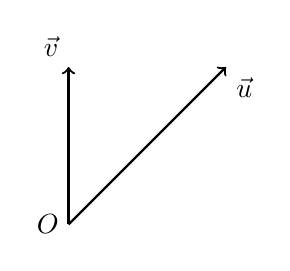
\begin{tikzpicture}[scale=2]
        \draw[black, thick, ->] (0, 0) -- (1, 1) node[anchor=north west] {$\vec u$};
        \draw[black, thick, ->] (0, 0) -- (0, 1) node[anchor=south east] {$\vec v$};
        \node[anchor=east] (0, 0) {$O$};
    \end{tikzpicture}
    \caption{Linearly independent}
    \end{figure}
\end{minipage}
\begin{minipage}{0.5 \textwidth}
    \begin{figure}[H]\tikzsetnextfilename{450}
    \centering
    \begin{tikzpicture}[scale=2]
        \draw[black, thick, ->] (0, 0) -- (1, 1) node[anchor=north west] {$\vec u$};
        \draw[black, thick, ->] (0, 0) -- (0.5, 0.5) node[anchor=south east] {$\vec v$};
        \node[anchor=east] (0, 0) {$O$};
    \end{tikzpicture}
    \caption{Linearly dependent}
    \end{figure}
\end{minipage}
In $\RR^3$, three vectors $\vec u$, $\vec v$ and $\vec w$ are linearly dependent if and only if they lie on the same line or plane (with their initial points at the origin).

\section{Basis and Dimension}

\begin{definition}
    A \vocab{basis} $S = \bc{\vec v_1, \dots, \vec v_r}$ for a linear space $V$ is a set of vectors such that
    \begin{itemize}
        \item $S$ spans $V$, and
        \item $S$ is linearly independent.
    \end{itemize}
\end{definition}

\begin{definition}
    Let $\vec e_1 = (1, 0, \dots, 0)$, $\vec e_2 = (0, 1, 0, \dots, 0)$, $\dots$, $\vec e_n = (0, \dots, 0, 1)$. The set $\bc{\vec e_1, \vec e_2, \dots, \vec e_n}$ is called the \vocab{standard basis} of $\RR^n$.
\end{definition}

\begin{sample}
    Show that the set \[S = \bc{\cveciv1010, \cveciv01{-1}2, \cveciv0221, \cveciv1001}\] is a basis for $\RR^4$.
\end{sample}
\begin{sampans}
    We first show that $S$ spans $\RR^4$. Consider $\vec v = \cvecivx{a}{b}{c}{d}$, where $a, b, c, d \in \RR$. Consider \[k_1 \cveciv1010 + k_2 \cveciv01{-1}2 + k_3 \cveciv0221 + k_4 \cveciv1001 = \cveciv{a}{b}{c}{d} \implies \begin{pmatrix}1 & 0 & 0 & 1\\ 0 & 1 & 2 & 0 \\ 1 & -1 & 2 & 0 \\ 0 & 2 & 1 & 1\end{pmatrix}\cveciv{k_1}{k_2}{k_3}{k_4} = \cveciv{a}{b}{c}{d}.\] Since the matrix on the LHS has non-zero determinant, every $\vec v$ can be expressed as a linear combination of the vectors of $S$. Thus, $S$ spans $\RR^4$.

    We now show that $S$ is linearly independent. Consider \[k_1 \cveciv1010 + k_2 \cveciv01{-1}2 + k_3 \cveciv0221 + k_4 \cveciv1001 = \cveciv0000 \implies \begin{pmatrix}1 & 0 & 0 & 1\\ 0 & 1 & 2 & 0 \\ 1 & -1 & 2 & 0 \\ 0 & 2 & 1 & 1\end{pmatrix}\cveciv{k_1}{k_2}{k_3}{k_4} = \cveciv0000.\] Since the matrix on the LHS has non-zero determinant, the equation has only the trivial solution. Thus, $S$ is linearly independent.
\end{sampans}

One particularly useful property about bases is that there is only one way to build a vector as a linear combination of given basis vector.

\begin{theorem}
    If $\bc{\vec v_1, \dots, \vec v_n}$ is a basis for a linear space $V$, then every vector $\vec v \in V$ can be expressed in the form $\vec v = k_1 \vec v_1 + \dots + k_n \vec v_n$ in exactly one way.
\end{theorem}

While a linear space can have many bases, the number of basis vectors must be the same. This number is called the dimension of $V$.

\begin{definition}
    The \vocab{dimension} of a non-zero linear space $V$ is the number of vectors in a basis for $V$, and is denoted $\Dim V$. By convention, we define the dimension of the zero linear space $\bc{\vec 0}$ to be 0.
\end{definition}

As an example, the linear space $\RR^n$ has dimension $n$ (recall that the standard basis consists of $n$ vectors).

We now state several remarks relating spans, linear independence and bases.

\begin{proposition}
    Let $V$ be a linear space with finite dimension $n$, and let $S \subseteq V$.
    \begin{itemize}
        \item If $\abs{S} > n$, then $S$ is linearly dependent.
        \item If $\abs{S} < n$, then $S$ cannot span $V$.
        \item If $\abs{S} = n$, then $S$ is a basis of $V$ if and only if $S$ is linearly independent if and only if $S$ spans $V$.
    \end{itemize}
\end{proposition}

The last property allows us to easily determine if a set is a basis of a linear space.

\begin{proposition}
    Let $V$ be a linear space with finite dimension $n$, and let $S \subseteq V$ be finite.
    \begin{itemize}
        \item If $S$ spans $V$ but is not a basis of $V$, then it can be reduced to a basis by removing certain vectors from $S$.
        \item If $S$ is linearly independent but not a basis of $V$, then it can be enlarged to a basis by adding in certain vectors from $V$.
    \end{itemize}
\end{proposition}

\section{Vector Spaces Associated with Matrices}

\subsection{Row Space, Column Space and Null Space}

Given an $m \times n$ matrix, there are three special subspaces of $\RR^m$ and $\RR^n$, namely the row space, column space and null space.

\begin{definition}
    Let $\mat A = (a)_{ij}$ be an $m \times n$ matrix. Define the \vocab{row vectors} of $\mat A$ to be \[\vec r_i = \begin{pmatrix}a_{i1} & a_{i2} & \dots & a_{in}\end{pmatrix}\trp.\] Then the \vocab{row space} of $\mat A$, denoted $\Row \mat A$, is the span of the row vectors of $\mat A$.
\end{definition}

Because it is the span of vectors in $\RR^n$, it is a subspace of $\RR^n$.

\begin{definition}
    Let $\mat A = (a)_{ij}$ be an $m \times n$ matrix. Define the \vocab{column vectors} of $\mat A$ to be \[\vec c_j = \begin{pmatrix}a_1j \\ a_2j \\ \vdots \\ a_mj \end{pmatrix}.\] Then the \vocab{column space} of $\mat A$, denoted $\Col \mat A$, is the span of the column vectors of $\mat A$.
\end{definition}

Because it is the span of vectors in $\RR^m$, it is a subspace of $\RR^m$.

\begin{definition}
    Let $\mat A$ be an $m \times n$ matrix. The \vocab{null space} of $\mat A$ is the solution set to the homogeneous system of equations $\mat A \vec x = \vec 0$, i.e. \[\bc{\vec x \in \RR^n : \mat A \vec x = \vec 0}.\]
\end{definition}

The null space is a subspace of $\RR^n$.

\begin{proposition}
    The row space is orthogonal to the null space.
\end{proposition}
\begin{proof}
    Let $\vec x$ be in the null space of $\mat A$, and let $\vec y$ be in the row space of $\mat A$. Let $\vec r_i$ be the $i$th row vector of $\mat A$. Then \[\mat A \vec x = \cveciii{\vec r_1 \dotp \vec x}{\vdots}{\vec r_m \dotp \vec x} = \cveciii0{\vdots}0.\] It follows that $\vec r_i \dotp \vec x = 0$ for all $1 \leq i \leq m$. Thus, \[\vec y \dotp \vec x = \bp{\sum_{i = 1}^m k_i \vec r_i} \dotp \vec x = \sum_{i = 1}^m k_i \bp{\vec r_i \dotp \vec x} = 0,\] so $\vec y$ and $\vec x$ are orthogonal. Thus, the row space is orthogonal to the null space.
\end{proof}

\subsection{Range Space and Kernel}

Let the linear transformation $T : \RR^n \to \RR^m$ be represented by the $m \times n$ matrix $\mat A$. In this section, we will introduce two special subspaces related to $T$, namely the range space and kernel of $T$. These two subspaces are equal to the column and null spaces of $\mat A$ respectively.

\begin{definition}
    The \vocab{range space} of $T$, denoted $\Range T$, consists of all vectors $\vec b$ such that $\mat A \vec x = \vec b$.
\end{definition}

\begin{proposition}
    $\Range T$ is equal to the column space of $\mat A$.
\end{proposition}
\begin{proof}
    Consider the equation $\mat A \vec x = \vec b$. Let $\vec c_i$ be the $i$th column vector of $\mat A$. Then we have \[\mat A \vec x =  \begin{pmatrix}\vec c_1 & \dots & \vec c_n\end{pmatrix} \cveciii{x_1}{\vdots}{x_n} = x_1 \vec c_1 + \dots + x_n \vec c_n = \vec b.\] Any vector $\vec b \in \Range T$ can be expressed as a linear combination of $\vec c_1, \dots, \vec c_n$. Thus, $\vec b$ is in the column space of $\mat A$. Likewise, any vector $\vec b$ in the column space of $\mat A$ is also in the range space of $T$. Thus, $\Range T$ is equal to the column space of $\mat A$.
\end{proof}

\begin{definition}
    The \vocab{kernel} of $T$, denoted $\Ker T$, is the set of all vectors $\vec x$ such that $\mat A \vec x = 0$.
\end{definition}

\begin{proposition}
    $\Ker T$ is equal to the null space of $\mat A$.
\end{proposition}
\begin{proof}
    Trivial.
\end{proof}

\subsection{Basis for Row Space}

\begin{definition}
    Two matrices $\mat A$ and $\mat B$ are said to be \vocab{row-equivalent} if their row spaces are the same.
\end{definition}

\begin{proposition}
    $\mat A$ and its REF/RREF are row-equivalent.
\end{proposition}
\begin{proof}
    Recall that an elementary row operation produces a new row that is a linear combination of the old rows. Thus, elementary row operations do not change the row space of a matrix. Since the REF/RREF of $\mat A$ can be obtained solely from elementary row operations, it follows that $\mat A$ and its REF/RREF are row-equivalent.
\end{proof}

This result allows us to easily find the basis of the row space of $\mat A$.

\begin{recipe}[Finding Basis of Row Space]
    Let $\mat B$ be the REF/RREF of $\mat A$. Then the non-zero row vectors in $\mat B$ form a basis for the row space of $\mat A$.
\end{recipe}

\begin{example}
    Let \[\mat A = \begin{pmatrix}1 & 2 & 3 & 4 & 5 \\ 6 & 7 & 8 & 9 & 10 \\ 11 & 12 & 13 & 14 & 15 \\ 16 & 17 & 18 & 19 & 21\end{pmatrix}.\] Its RREF is given by \[\begin{pmatrix}1 & 0 & -1 & -2 & 0 \\ 0 & 1 & 2 & 3 & 0 \\ 0 & 0 & 0 & 0 & 1 \\ 0 & 0 & 0 & 0 & 0\end{pmatrix}.\] Thus, a row space basis of $\mat A$ is \[\bc{\begin{pmatrix}1 \\ 0 \\ -1 \\ -2 \\ 0\end{pmatrix}, \begin{pmatrix}0 \\ 1 \\ 2 \\ 3 \\ 0\end{pmatrix}, \begin{pmatrix}0 \\ 0 \\ 0 \\ 0 \\ 1\end{pmatrix}}.\]
\end{example}

\subsection{Basis for Column Space}

One way of finding a basis for the column space of $\mat A$ would be to find a basis for the row space of $\mat A \trp$. However, there is a much simpler approach, which we now derive.

\begin{proposition}\label{prop:lin-alg:row-lindep}
    Row operations do not change the linear dependence on columns.
\end{proposition}
\begin{proof}
    Suppose we have a matrix $\mat A = \begin{pmatrix}\vec c_1 & \dots & \vec c_n\end{pmatrix}$. The linear independence of the column vectors depends on the solution set $\vec x$ to the equation \[x_1 \vec c_1 + \dots x_n \vec c_n = 0 \implies \mat A \vec x = 0.\] Suppose now that we perform row operations on $\mat A$ to obtain a new matrix $\mat A'$. By writing the above equation as an augmented matrix, we see that the row operations do not change the solution set $\vec x$! \[\begin{pmatrix}[c|c]\mat A & \vec 0\end{pmatrix} \rightarrow \begin{pmatrix}[c|c]\mat A' & \vec 0\end{pmatrix} \implies x_1 \vec c_1' + \dots + x_n \vec c_n' = 0.\] Thus, if $\vec c_i$ and $\vec c_j$ were originally linearly independent, the corresponding columns $\vec c_i'$ and $\vec c_j'$ will remain linearly independent. Likewise for columns that were originally linearly dependent. Thus, row operations do not change linear dependence on columns.
\end{proof}

Note however, that row operations do not preserve the column space of $\mat A$. For instance, \[\begin{pmatrix}1 & 0 \\ 0 & 0\end{pmatrix} \quad \tand \quad \begin{pmatrix}0 & 0 \\ 1 & 0\end{pmatrix}\] are row-equivalent, but their column spaces are entirely different.

As a consequence of the above result, we obtain the following corollaries:
\begin{corollary}
    If $\mat A$ and $\mat B$ are row-equivalent, a given set of columns of $\mat A$ forms a basis for $\Col{\mat A}$ if and only if the corresponding set of columns of $\mat B$ forms a basis for $\Col{\mat B}$.
\end{corollary}

With this, we have our standard procedure for finding a basis for the column space of $\mat A$:

\begin{recipe}[Finding Basis of Column Space]
    Let $\mat B$ be the REF/RREF of $\mat A$. Look at the columns of $\mat B$ with a leading entry. Then the corresponding columns of $\mat A$ form a basis of $\Col{\mat A}$.
\end{recipe}

\begin{example}
    Let \[\mat A = \begin{pmatrix}1 & 2 & 3 & 4 & 5 \\ 6 & 7 & 8 & 9 & 10 \\ 11 & 12 & 13 & 14 & 15 \\ 16 & 17 & 18 & 19 & 21\end{pmatrix}.\] Its RREF is given by \[\mat B = \begin{pmatrix}\boxed{1} & 0 & -1 & -2 & 0 \\ 0 & \boxed{1} & 2 & 3 & 0 \\ 0 & 0 & 0 & 0 & \boxed{1} \\ 0 & 0 & 0 & 0 & 0\end{pmatrix}.\] The first, second and fifth columns of $\mat B$ contain a leading entry. Thus, the first, second and fifth columns of $\mat A$ form a basis of $\Col{\mat A}$: \[\bc{\cveciv16{11}{16}, \cveciv27{12}{17}, \cveciv5{10}{15}{21}}.\]
\end{example}

\subsection{Basis for Null Space}

In the proof of Proposition~\ref{prop:lin-alg:row-lindep}, we saw how row operations do not change the solution set of the equation $\mat A \vec x = \vec 0$. Hence, if $\mat B$ is the REF/RREF of $\mat A$, then the equations $\mat A \vec x = 0$ and $\mat B \vec x = \vec 0$ will have the same solution set. 

\begin{recipe}[Finding Basis of Null Space]
    Let $\mat B$ be the REF/RREF of $\mat A$. Then the null space of $\mat A$ is the solution set $\vec x$ of $\mat B \vec x = \vec 0$.
\end{recipe}

\begin{example}
    Let \[\mat A = \begin{pmatrix}1 & 2 & 3 & 4 & 5 \\ 6 & 7 & 8 & 9 & 10 \\ 11 & 12 & 13 & 14 & 15 \\ 16 & 17 & 18 & 19 & 21\end{pmatrix}.\] Its RREF is given by \[\mat B = \begin{pmatrix}1 & 0 & -1 & -2 & 0 \\ 0 & 1 & 2 & 3 & 0 \\ 0 & 0 & 0 & 0 & 1 \\ 0 & 0 & 0 & 0 & 0\end{pmatrix}.\] We notice that columns 3 and 4 do not have leading entries. The variables corresponding to these columns can thus be set as free variables. \[\mat B \vec x = \begin{pmatrix}1 & 0 & -1 & -2 & 0 \\ 0 & 1 & 2 & 3 & 0 \\ 0 & 0 & 0 & 0 & 1 \\ 0 & 0 & 0 & 0 & 0\end{pmatrix} \begin{pmatrix}x_1 \\ x_2 \\ x_3 \\ x_4 \\ x_5 \end{pmatrix} = \begin{pmatrix}0 \\ 0 \\ 0 \\ 0 \\ 0\end{pmatrix} \implies \systeme{x_1 - x_3 - 2x_4 = 0, x_2 + 2x_3 + 3x_4 = 0, x_5 = 0}.\] Setting $x_3 = s$ and $x_4 = t$, we have \[\begin{pmatrix}x_1 \\ x_2 \\ x_3 \\ x_4 \\ x_5 \end{pmatrix} = \begin{pmatrix}s + 2t \\ -2s - 3t \\ s \\ t \\ 0 \end{pmatrix} = s \begin{pmatrix}1 \\ -2 \\ 1 \\ 0 \\ 0\end{pmatrix} + t \begin{pmatrix}2 \\ -3 \\ 0 \\ 1 \\ 0 \end{pmatrix}.\] Thus, the basis of the null space of $\mat A$ is \[\bc{\begin{pmatrix}1 \\ -2 \\ 1 \\ 0 \\ 0\end{pmatrix}, \begin{pmatrix}2 \\ -3 \\ 0 \\ 1 \\ 0 \end{pmatrix}}.\]
\end{example}

\section{Rank and Nullity for Matrices}

\begin{definition}
    The \vocab{row rank} of $\mat A$ is the dimension of the row space of $\mat A$. The \vocab{column rank} of $\mat A$ is the dimension of the column space of $\mat A$.
\end{definition}

\begin{proposition}
    Row and column ranks are equal.
\end{proposition}
\begin{proof}
    Recall the procedure we took to find the basis for the row and column space of a matrix:
    \begin{itemize}
        \item The column space basis consists of columns in the original matrix corresponding to the leading entries in the REF/RREF.
        \item The row space basis consists of the rows of the REF/RREF corresponding to the leading entries.
    \end{itemize}
    Since each leading entry corresponds to exactly one row and one column, the sizes of the row and column spaces bases must be equal. Hence, the row and column ranks are equal.
\end{proof}

We give this common value a special name:

\begin{definition}
    The \vocab{rank} of $\mat A$ is the dimension of the row/column space of $\mat A$. It is denoted by $\Rank \mat A$.
\end{definition}

Let $\mat A$ be an $m \times n$ matrix. Because the row rank is at most $m$, and the column rank is at most $n$, we have that $\Rank \mat A \leq \min{m, n}$. If equality is achieved, we give $\mat A$ a special name:

\begin{definition}
    Let $\mat A$ be an $m \times n$ matrix. If $\Rank \mat A = \min{m, n}$, we say $\mat A$ has \vocab{full rank}.
\end{definition}

\begin{proposition}
    $\Rank{\mat A \mat B} \leq \min{\Rank \mat A, \Rank \mat B}$.
\end{proposition}
\begin{proof}
    Every column in $\mat A \mat B$ can be expressed as a linear combination of the columns of $\mat A$, so $\Col{\mat A \mat B} \subseteq \Col \mat A$. Taking dimensions, we see that \[\Rank{\mat A \mat B} = \dim \Col{\mat A \mat B} \leq \dim \Col \mat A = \Rank \mat A.\] Similarly, every row in $\mat A \mat B$ can be expressed as a linear combination of the rows of $\mat B$, so $\Row{\mat A \mat B} \subseteq \Row \mat B$. Taking dimensions, \[\Rank{\mat A \mat B} = \dim \Row{\mat A \mat B} \leq \dim \Row \mat B = \Rank \mat B.\] Combining these two inequalities gives us what we want.
\end{proof}

We can slightly extend the above result:

\begin{proposition}
    If $\mat B$ is an invertible $n \times n$ matrix, then $\Rank{\mat A \mat B} = \Rank{\mat B \mat A} = \Rank \mat A$ for all $n \times n$ matrices $\mat A$.
\end{proposition}
\begin{proof}
    Observe that \[\Rank \mat A = \Rank{\mat A \mat B \mat B^{-1}} \leq \Rank{\mat A \mat B} \leq \Rank \mat A,\] so $\Rank{\mat A \mat B} = \Rank \mat A$. Similarly, \[\Rank \mat A = \Rank{\mat B^{-1} \mat B \mat A} \leq \Rank{\mat B \mat A} \leq \Rank \mat A.\] so $\Rank{\mat B \mat A} = \Rank \mat A$.
\end{proof}

\begin{definition}
    The \vocab{nullity} of $\mat A$ is the dimension of the null space of $\mat A$. It is denoted by $\Nullity \mat A$.
\end{definition}

\begin{theorem}[Rank-Nullity Theorem]
    For an $m \times n$ matrix $\mat A$, \[\Rank \mat A + \Nullity \mat A = \text{number of columns of $\mat A$, } n.\]
\end{theorem}
\begin{proof}
    $\Rank \mat A$ is equal to the number of columns in the RREF that contains a leading entry, while $\Nullity \mat A$ is equal to the number of columns in the RREF that does not contain a leading entry. Thus, their sum must be the number of columns in the RREF, which is $n$.
\end{proof}

We can determine the number of solutions to a system of linear equations using the rank of its corresponding matrix:

\begin{recipe}[Finding Number of Solutions]
    Let $\mat A \vec x = \vec b$ be a system of linear equations in $n$ variables. Then
    \begin{itemize}
        \item if $\Rank \mat A = \Rank \begin{pmatrix}[c|c] \mat A & \vec b\end{pmatrix} = n$, the system if consistent and has a unique solution.
        \item if $\Rank \mat A = \Rank \begin{pmatrix}[c|c] \mat A & \vec b\end{pmatrix} < n$, then the system is consistent and has an infinite number of solutions.
        \item if $\Rank \mat A < \Rank \begin{pmatrix}[c|c] \mat A & \vec b\end{pmatrix}$, then the system is inconsistent and thus has no solution.
    \end{itemize}
\end{recipe}

In the case where the system is consistent, we can apply the following result to find all possible solutions to the system:

\begin{proposition}
    If $\vec x_p$ is a particular solution of a consistent non-homogeneous system $\mat A \vec x = \vec b$, then every solution of the system can be written in the form $\vec x = \vec x_p + \vec x_h$, where $\vec x_h$ is a solution to the corresponding homogeneous system $\mat A \vec x = \vec 0$.
\end{proposition}
\begin{proof}
    Let $\vec x_p$ be a fixed solution of $\mat A \vec x = \vec b$, and let $\vec x$ be an arbitrary solution. Then \[\mat A \vec x = \vec b \quad \tand \quad \mat A \vec x_p = \vec b.\] Subtracting these equations yields \[\mat A \bp{\vec x - \vec x_p} = \vec 0,\] so $\vec x - \vec x_p$ is a solution of the homogeneous system $\mat A \vec x = \vec 0$. Let $\bc{\vec v_1, \dots, \vec v_k}$ form a basis for the null space of $\mat A$. Then there exist $c_1, \dots, c_k \in \RR$ such that \[\vec x - \vec x_p = c_1 \vec v_1 + \dots + c_k \vec v_k.\] Letting $\vec x_h = c_1 \vec v_1 + \dots + c_k \vec v_k$, we see that \[\vec x = \vec x_p + \vec x_h\] as desired.
\end{proof}

\section{Rank and Nullity for Linear Transformations}

\begin{definition}
    Let $T$ be a linear transformation. The dimension of the range of $T$ is called the \vocab{rank} of $T$ and the dimension of the kernel of $T$ is called the \vocab{nullity} of $T$.
\end{definition}

\begin{theorem}[Rank-Nullity Theorem for Linear Transformations]
    For a linear transformation $T : \RR^m \to \RR^n$, where $T(\vec x) = \mat A \vec x$, we have \[\Rank T + \Nullity T = \Rank \mat A + \Nullity \mat A = n.\]
\end{theorem}
\begin{proof}
    Recall that the range of $T$ is the column space of $\mat A$ and the kernel of $T$ is the null space of $\mat A$. Hence, \[\Rank T = \Dim \Range T = \Dim \Col \mat A = \Rank \mat A\] and \[\Nullity T = \Dim \Ker T = \Dim{\text{null space of $\mat A$}} = \Nullity \mat A.\] By the Rank-Nullity Theorem for matrices, we have \[\Rank T + \Nullity T = \Rank \mat A + \Nullity \mat A = n.\]
\end{proof}